\section{Applications of Integrals}
\label{sec:integral-applications}

% From Sections 3.7 and 3.6

\subsection{Consumer and Producer Surplus}
Two of the most fundamental concepts in economics are {\bf supply}\index{Supply} and {\bf demand}\index{Demand}.
\begin{definition}[Supply and Demand]
Suppose some item is bought and sold for a price. The {\bf supply} of the item is the quantity, $q$, of the item that is available for sale on some market at some price $p$. The {\bf demand} of the item is the quantity, $q$, of the itme that buyers are willing to buy at some price $p$.
\end{definition}
To get a feel for how supply and demand change as price and quantities change, consider Figure \ref{fig:5-8-supplyDemand}, which shows demand and supply curves for a product. Which is which?

\begin{figure}[!ht]
  \centering
    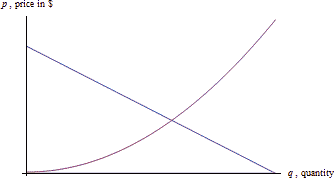
\includegraphics[width=0.4\textwidth]{img/chap5/image062.png}
    \caption{Supply and demand curves for $q$ items.}
    \label{fig:5-8-supplyDemand}
\end{figure}
The {\bf demand curve}\index{Demand curve} is decreasing -- lower prices are associated with higher quantities demanded, higher prices are associated with lower quantities demanded. Demand curves are often shown as if they were linear, but there's no reason they have to be.

The {\bf supply curve}\index{Supply curve} is increasing -- lower prices are associated with lower supply, and higher prices are associated with higher quantities supplied.

The point where the demand and supply curve cross is called the {\bf equilibrium point}\index{Equilibrium point} $(q^{*},p^{*})$; $p^{*}$ is the price at which supply and demand are exactly the same.

\begin{figure}[!ht]
  \centering
    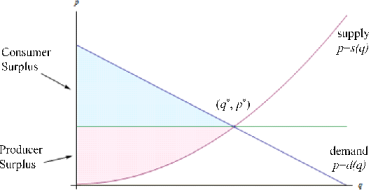
\includegraphics[width=0.4\textwidth]{img/chap5/image063.png}
    \caption{Equilibrium point on supply and demand curves.}
    \label{fig:5-8-equilibrium}
\end{figure}
Suppose that the price is set at the {\bf equilibrium price}\index{Equilibrium price}, $p^{*}$, so that the quantity demanded equals the quantity supplied. Now think about the folks who are represented on the left of the equilibrium point. The consumers on the left would have been willing to pay a higher price than they ended up having to pay, so the equilibrium price saved them money. On the other hand, the producers represented on the left would have been willing to supply these goods for a lower price -- they made more money than they expected to. Both of these groups ended up with extra cash in their pockets!

Graphically, the amount of extra money that ended up in consumers' pockets is the area between the demand curve and the horizontal line $y = p^{*}$. This is the difference in price, summed up over all the consumers who spent less than they expected to -- a definite integral. Notice that since the area under the horizontal line is a rectangle, we can simplify the area integral:
$$\int_0^{q^{*}}(d(q)-p^{*})\,dq = \int_0^{q^{*}}d(q)\,dq-\int_0^{q^{*}}p^{*}\,dq = \int_0^{q^{*}}d(q)\,dq - p^{*}q^{*} \enspace .$$
The amount of extra money that ended up in producers' pockets is the area between the supply curve and the horizontal line at p*. This is the difference in price, summed up over all the producers who received more than they expected to. Similar to consumer surplus, this integral can be simplified:
$$\int_0^{q^{*}}(p^{*} - s(q))\,dq = \int_0^{q^{*}}p^{*}\,dq - \int_0^{q^{*}}s(q)\,dq = p^{*}q^{*} - \int_0^{q^{*}}s(q)\,dq \enspace .$$
\begin{definition}[Consumer and Producer Surplus]
Given a demand function $p=d(q)$ and a supply function $p=s(q)$, and the equilibrium point $(q^{*},p^{*})$.
The {\bf consumer surplus}\index{Consumer surplus}\index{Surplus!consumer} is
$$\int_0^{q^{*}}d(q)\,dq - p^{*}q^{*} \enspace .$$
The {\bf producer surplus}\index{Producer surplus}\index{Surplus!producer} is
$$p^{*}q^{*} - \int_0^{q^{*}}s(q)\,dq.$$
The sum of the consumer surplus and producer surplus is the {\bf total gains from trade}\index{Total gains from trade}.
\end{definition}
What are the units of consumer and producer surplus? The units are (price per item)(quantity of items) $=$ money!

\begin{example}
Suppose the demand for a product is given by $p=d(q)=-0.8q+150$ and the supply for the same product is given by $p=s(q)=5.2q$. For both functions, $q$ is the quantity and $p$ is the price, in dollars.
\begin{enumerate}[label=(\alph*)]
  \item Find the equilibrium point.

  \begin{solution}
The equilibrium point is where the supply and demand functions are equal. Solving $-0.8q+150=5.2q$ gives $q=25$.
  \end{solution}
  \item Find the consumer surplus at the equilibrium price.

  \begin{solution}
    The consumer surplus is
    $$\int_0^{25}(-0.8q+150)\,dq - (130)(25) = \$250 \enspace .$$
  \end{solution}
  \item Find the producer surplus at the equilibrium price.

\begin{solution}
  The producer surplus is
  $$(130)(25) - \int_0^{25}5.2q\,dq = \$1625 \enspace .$$
  \end{solution}
\end{enumerate}
\end{example}

\begin{example}
Tables \ref{tab:5-8-demand} and \ref{tab:5-8-supply} show information about the demand and supply functions for a product. For both functions, $q$ is the quantity and $p$ is the price, in dollars.

\begin{table}[ht!]
    \centering
    \begin{tabular}{l*{8}{r}}
    \toprule
    {\bf Quantity:} $q$ (items) & 0 & 	100	 & 200	 & 300	 & 400	 & 500	 & 600	 & 700\tabularnewline
    \midrule
    {\bf Price:} $p$ (\$) & 70 & 	61 & 	53 & 	46 & 	40 & 	35 & 	31 & 	28\tabularnewline
    \bottomrule
    \end{tabular}
    \caption{Demand or supply of a product.}
    \label{tab:5-8-demand}
\end{table}
\begin{table}[ht!]
    \centering
    \begin{tabular}{l*{8}{r}}
    \toprule
    {\bf Quantity:} $q$ (items) & 0 & 	100	 & 200	 & 300	 & 400	 & 500	 & 600	 & 700\tabularnewline
    \midrule
    {\bf Price:} $p$ (\$)       & 14 & 	21 & 	28 & 	33 & 	40 & 	47 & 	54 & 	61\tabularnewline
    \bottomrule
    \end{tabular}
    \caption{Demand or supply of a product.}
    \label{tab:5-8-supply}
\end{table}
  \begin{enumerate}[label=(\alph*)]
    \item Which is which? That is, which table represents demand and which represents supply?

    \begin{solution}
      Table \ref{tab:5-8-demand} shows decreasing price associated with increasing quantity, so that is the demand function. Table \ref{tab:5-8-supply} shows increasing price associated with increasing quantity, so that is the supply function.
    \end{solution}
    \item What is the equilibrium price and quantity?

    \begin{solution}
For both functions, $q=400$ is associated with $p=40$, so the equilibrium price is \$40 and the equilibrium quantity is 400 units. Notice that we were lucky here, because the equilibrium point is actually one of the points shown. In many cases with a table, we would have to estimate.
    \end{solution}
    \item Find the consumer and producer surplus at the equilibrium price.

    \begin{solution}
      The consumer surplus uses the demand function, which comes from the first table. We'll have to approximate the value of the integral using rectangles. There are 4 rectangles, and let's choose to use left endpoints.

      The consumer surplus is
      $$\int_0^{400}(demand)\,dq - (40)(400) \approx   (100)(70+61+53+46)-(40)(400)=\$7000 \enspace .$$
      So the consumer surplus is about \$7000.

      The producer surplus uses the supply function, which comes from the second table. Let's choose to use left endpoints for this integral also.

      The producer surplus is
      $$(40)(400) - \int_0^{400}(supply)\,dq\approx   (40)(400)-(100)(14+21+28+33)=\$6400 \enspace ,$$
      so the producer surplus is about \$6400.
    \end{solution}
  \end{enumerate}
\end{example}

\subsection{Continuous Income Stream}\index{Income stream}
In precalculus, you learned about compound interest\index{Compound interest}\index{Interest!compound} in that really simple situation where you made a single deposit into an interest-bearing account and let it sit undisturbed, earning interest, for some period of time. Recall:

\begin{definition}[Compound Interest Formulas]
Let $P$ be the principal\index{Principal} (initial investment), $r$ be the annual interest rate expressed as a decimal, and $A(t)$ be the amount in the account after $t$ years.

\noindent{\bf Compounding $n$ times per year:}
$$A(t)=P\left(1+\frac{r}{n}\right)^{nt}$$
\noindent{\bf Compounding continuously:}
$$A(t)=Pe^{rt}$$
If you're using this formula to find what an account will be worth in the future, $t>0$ and $A(t)$ is called the {|bf future value}\index{Future value}\index{Value!future}.

If you're using the formula to find what you need to deposit today to have a certain value $P$ sometime in the future, $t<0$ and $A(t)$ is called the {\bf present value}\index{Present value}\index{Value!present}.
\end{definition}

You may also have learned somewhat more complicated annuity formulas to deal with slightly more complicated situations -- where you make equal deposits equally spaced in time.

But real life is not usually so neat.

Calculus allows us to handle situations where deposits are flowing continuously into an account that earns interest. As long as we can model the flow of income with a function, we can use a definite integral to calculate the present and future value of a continuous income stream. The idea here is that each little bit of income in the future needs to be multiplied by the exponential function to bring it back to the present, and then we'll add them all up (a definite integral).

\begin{definition}[Continuous Income Stream]\index{Income stream}
Suppose money can earn interest at an annual interest rate of $r$, compounded continuously. Let $F(t)$ be a continuous income function (in dollars per year) that applies between year $0$ and year $T$.

Then the {\bf present value}\index{Present value}\index{Value!present} of that income stream is given by
$$PV=\int_0^T F(t)e^{-rt}\,dt \enspace.$$
The {\bf future value}\index{Future value}\index{Value!future} can be computed by the ordinary compound interest formula
$$FV=PVe^{rt} \enspace .$$
\end{definition}
This is a useful way to compare two investments -- find the present value of each to see which is worth more today.

\begin{example}
You have an opportunity to buy a business that will earn \$75,000 per year continuously over the next eight years. Money can earn 2.8\% per year, compounded continuously. Is this business worth its purchase price of \$630,000?

\begin{solution}
  First, please note that we still have to make some simplifying assumptions. We have to assume that the interest rates are going to remain constant for that entire eight years. We also have to assume that the \$75,000 per year is coming in continuously, like a faucet dripping dollars into the business. Neither of these assumptions might be accurate.

But moving on, the present value of the \$630,000 is, well, \$630,000. This is one investment, where we put our \$630,000 in the bank and let it sit there.

To find the present value of the business, we think of it as an income stream. The function F(t) in this case is a constant \$75,000 dollars per year, so $F(t)=75,000$. The interest rate is 2.8\% and the term we're interested in is 8 years, so $r=.028$, and $T=8$:
$$PV = \int_0^8 75000e^{-0.028t}\,dt\approx   537548.75 \enspace .$$
The present value of the business is about \$537{,}500, which is less than the \$630,000 asking price, so this is not a good deal.
\end{solution}\end{example}

While this integral could have been done using substitution, for many of the integrals in this section we don't have the techniques to use antiderivatives or, in some cases, no antiderivative exists. Technology will work quickly, and it will give you an answer that is good enough.

\begin{example}
A company is considering purchasing a new machine for its production floor. The machine costs \$65,000. The company estimates that the additional income from the machine will be a constant \$7000 for the first year, then will increase by \$800 each year after that. In order to buy the machine, the company needs to be convinced that it will pay for itself by the end of 8 years with this additional income. Money can earn 1.7\% per year, compounded continuously. Should the company buy the machine?

\begin{solution}
  We'll assume that the income will come in continuously over the 8 years. We'll also assume that interest rates will remain constant over that 8-year time period.

We're interested in the present value of the machine, which we will compare to its \$65,000 price tag. Let $t$ be the time, in years, since the purchase of the machine. The income from the machine is different depending on the time.

From $t=0$ to $t=1$ (the first year), the income is constant \$7000 per year. From $t=1$ to $t=8$, the income is increasing by \$800 each year; the income flow function $F(t)$ will be $F(t)=7000+800(t-1)=6200+800t$. To find the present value, we'll have to divide the integral into the two pieces, one for each of the functions:
$$PV=\int_0^1 7000e^{-0.017t}\,dt + \int_1^8 (6200+800t)e^{-0.017t}\,dt\approx   70166 \enspace.$$
The present value is greater than the cost of the machine, so the company should buy the machine.
\end{solution}\end{example}

\subsection{Average Value}
We know the average of $n$ numbers $a_1, a_2,\ldots, a_n$ is their sum divided by $n$. But what if we need to find the average temperature over a day's time -- there are too many possible temperatures to add them up! This is a job for the definite integral.

% From Section 3.6.
\begin{definition}[Average Value]
The average value of a function $f(x)$ on the interval $[a,b]$ is given by
$$\frac{1}{b-a}\int_a^b f(x)\,dx \enspace .$$
\end{definition}

The average value of a positive function $f(x)$ has a nice geometric interpretation. Imagine that the area under the curve $y=f(x)$ (graph (a) in Figure \ref{fig:5-8-liquid}) is a liquid that can leak through the graph to form a rectangle with the same area (graph (b) in Figure \ref{fig:5-8-liquid}).

\begin{figure}[!ht]
  \centering
    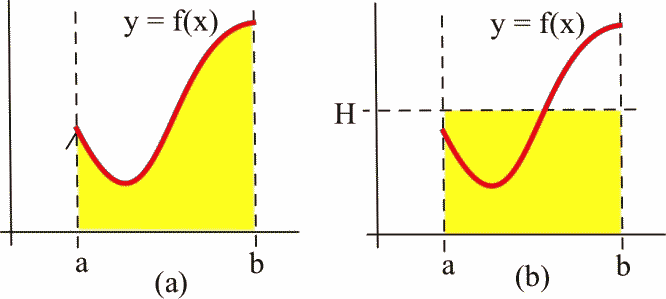
\includegraphics[width=0.6\textwidth]{img/chap5/image053.png}
    \caption{Visualizing average value}
    \label{fig:5-8-liquid}
\end{figure}

If the height of the rectangle is $H$, then the area of the rectangle is $H\cdot(b-a)$. We know the area of the rectangle is the same as the area under $y=f(x)$ between $x=a$ and $x=b$ so $H\cdot(b-a)=\int_a^b f(x)\,dx$. Then
$$H = \frac{1}{b-a}\int_a^bf(x)\,dx\enspace ,$$
the average value of $f(x)$ on the closed interval $[a,b]$.

The average value of a positive function $f(x)$ is the height $H$ of the rectangle whose area is the same as the area under $y=f(x)$.

\begin{example}
During a 9 hour work day, the production rate at time $t$ hours after the start of the shift was given by the function $r(t)=5+\sqrt{t}$ cars per hour. Find the average hourly production rate.

\begin{solution}
The average hourly production is $\displaystyle\frac{1}{9-0}\displaystyle\int_0^9\left(5+\sqrt{t}\right)\,dt=7$ cars per hour.
\end{solution}\end{example}

A note about the units -- remember that the definite integral has units (cars per hour)$\cdot$(hours) $=$ cars. But the $\dfrac{1}{b-a}$ in front has units 1hours -- the units of the average value are cars per hour, just what we expect an average rate to be.

\begin{note}
In general, the average value of a function will have the same units as the integrand.
\end{note}

Function averages, involving means and more complicated averages, are used to smooth data so that underlying patterns are more obvious and to remove high frequency noise from signals. In these situations, the original function $f(x)$ is replaced by some average of $f(x)$. If $f(x)$ is rather jagged time data, then the ten year average of $f(x)$ is the integral $g(x) = \displaystyle\frac{1}{10}\int_{x-5}^{x+5}f(t)\,dt$, an average of $f(x)$ over 5 units on each side of $x$.

For example, Figure \ref{fig:5-8-temp} shows the graphs of a Monthly Average (rather ``noisy" data) of surface temperature data, an Annual Average (still rather jagged), and a Five Year Average (a much smoother function).

\begin{figure}[!ht]
  \centering
    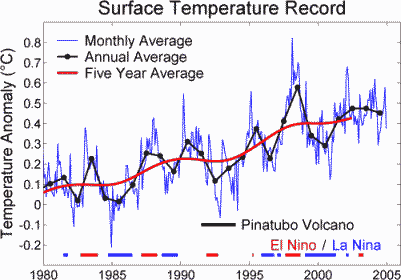
\includegraphics[width=0.4\textwidth]{img/chap5/image054.png}
    \caption{Image prepared by Robert A. Rohde,\\ http://commons.wikimedia.org/wiki/File:Short\_Instrumental\_Temperature\_Record.png.}
    \label{fig:5-8-temp}
\end{figure}
Typically the average function reveals the pattern much more clearly than the original data. This use of a {\bf moving average}\index{Moving average} value of noisy data (weather information, stock prices) is a very common, especially data that is a {\bf time series}\index{Time series}, data that is a function of time.

\begin{example}
The graph in Figure \ref{fig:5-8-reservoir} shows the volume of water in a reservoir over a 12 hour period. Estimate the average amount of water in the reservoir over this period.

\begin{figure}[!ht]
  \centering
    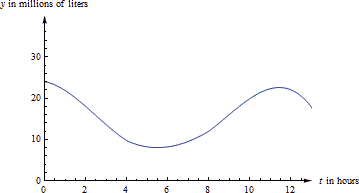
\includegraphics[width=0.4\textwidth]{img/chap5/image055.png}
    \caption{Volume of water in a reservoir over a 12-hour span.}
    \label{fig:5-8-reservoir}
\end{figure}
\begin{solution}
If $V(t)$ is the volume of the water (in millions of liters) after $t$ hours, then the average amount is $\dfrac{1}{12}\displaystyle\int_0^{12}V(t)\,dt$. In order to find the definite integral, we'll have to estimate. Let's use 6 rectangles and take the heights from their right edges (there's nothing special about using 6 rectangles or right edges -- other choices would still give you a valid estimate).

\begin{figure}[!ht]
  \centering
    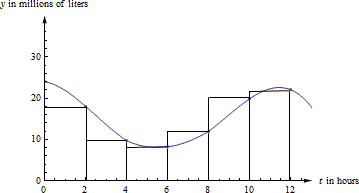
\includegraphics[width=0.4\textwidth]{img/chap5/image056.png}
    \caption{Estimating the average volume of water in a reservoir.}
    \label{fig:5-8-reservoir}
\end{figure}

The estimate of the integral is
$$\int_0^{12}V(t)\,dt\approx   (18)(2)+(9.7)(2)+(8.2)(2)+(12)(2)+(19.9)(2)+(22)(2)=179.6 \enspace .$$
The units of this integral are millions of liters. So our estimate of the average volume is $112\cdot 179.6 \approx 15$ million liters. (The estimate might change a little depending on how we estimate the function values from the graph.)

In Figure \ref{fig:5-8-reservoiravg}, you can see the same graph as the one in Figure \ref{fig:5-8-reservoir} with the line $y=15$ drawn in. The area under the curve and the area under the rectangle are (approximately) the same; this confirms that our solution is plausible and makes sense.

\begin{figure}[!ht]
  \centering
    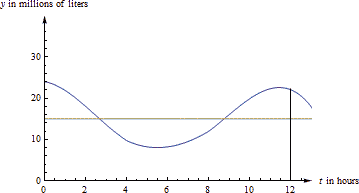
\includegraphics[width=0.4\textwidth]{img/chap5/image057.png}
    \caption{Estimating the average volume of water in a reservoir.}
    \label{fig:5-8-reservoiravg}
\end{figure}

In fact, that would be a different way to estimate the average value. We could have estimated the placement of the horizontal line so that the area under the curve and under the line were equal.
\end{solution}\end{example}

\subsection{Area Between Curves}
We have already used integrals to find the area between the graph of a function and the horizontal axis. Integrals can also be used to find the area between two graphs.

If $f(x) \geq g(x)$ for all $x \in [a,b]$, then we can approximate the area between the curves $y=f(x)$ and $y=g(x)$ between $x=a$ and $x=b$ by partitioning the interval $[a,b]$ and forming a Riemann sum, as shown in Figure \ref{fig:5-8-abc}. The height of the $i$th rectangle is top $-$ bottom, or $f(c_i)-g(c_i)$ so the area of the $i$-th rectangle is (height)$\cdot$(base) $= (f(c_i)-g(c_i))\Delta x$. Adding up these rectangles gives an approximation of the total area as $\displaystyle\sum_{i=1}^n(f(c_i)-g(c_i))\Delta x$, a Riemann sum.

\begin{figure}[!ht]
  \centering
    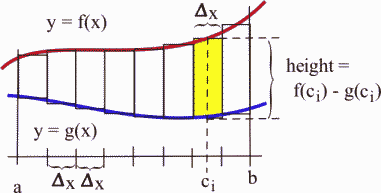
\includegraphics[width=0.4\textwidth]{img/chap5/image049.png}
    \caption{Estimating the area between two curves.}
    \label{fig:5-8-abc}
\end{figure}
The limit of this Riemann sum, as the number of rectangles gets larger and their width gets smaller, is the definite integral $\displaystyle\int_a^b(f(x)-g(x))\,dx$.

\begin{theorem}[Area Between Two Curves]
The area between two curves $f(x)$ and $g(x)$, where $f(x)\geq g(x)$, between $x=a$ and $x=b$ is
$$\int_a^b(f(x)-g(x))\,dx \enspace .$$
The integrand is top $-$ bottom. Make a graph or use test values to be sure which curve is which.
\end{theorem}
\begin{example}
\label{ex:5-8-3}
Find the area bounded between the graphs of $f(x)=x$ and $g(x)=3$ for $1\leq x\leq 4$.

\begin{figure}[!ht]
  \centering
    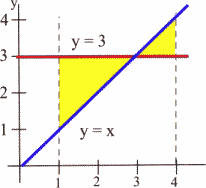
\includegraphics[width=0.3\textwidth]{img/chap5/image050.png}
    \caption{Graph for example \ref{ex:5-8-3}.}
    \label{fig:5-8-ex3}
\end{figure}

\begin{solution}
Always start with a graph so you can see which graph is the top and which is the bottom. In this example, the two curves cross, and they change positions; we'll need to split the area into two pieces. Geometrically, we can see that the area is $2 + 0.5 = 2.5$.

Writing the area as a sum of definite integrals, we get
$$\text{Area} = \int_1^3(3-x)\,dx + \int_3^4(x-3)\,dx \enspace .$$
These integrals are easy to evaluate using antiderivatives:
  \begin{align*}
    \int_1^3(3-x)\,dx &= \left.3x-\frac{x^2}{2}\right|_1^3 \\
    &= \left(9-\frac{9}{2}\right) - \left(3-\frac{1}{2}\right) \\
    &= 2
  \end{align*}
  \begin{align*}
    \int_3^4(x-3)\,dx &= \left.\frac{x^2}{2}-3x\right|_3^4 \\
    &= \left(\frac{16}{2}-12\right) - \left(\frac{9}{2}-9\right)\\
    &= \frac{1}{2}
  \end{align*}
The sum of these two integrals tells us that the total area between $y=f(x)$ and $y=g(x)$ over the interval $[1, 4]$ is 2.5 square units, which we already knew from the picture.
\end{solution}\end{example}

Note that the single integral $\displaystyle\int_1^3(3-x)\,dx=1.5$ is not the area we want in the last example. The value of the integral is 1.5, and the value of the area is 2.5. That's because the triangle on the right is below the $x$-axis. The graph of $y=x$ is above the graph of $y=3$, so the integrand $3-x$ is negative; in the definite integral, the area of that triangle comes in with a negative sign.

In this example, it was easy to see exactly where the two curves crossed so we could break the region into the two pieces to figure separately. In other examples, you might need to solve an equation to find where the curves cross.

\begin{example}
  \label{ex:5-8-4}
Two objects, $A$ and $B$, start from the same location and travel along the same path with velocities $v_A(t)=t+3$ and $v_B(t)=t^2-4t+3$ meters per second. How far ahead is $A$ after 3 seconds?

\begin{figure}[!ht]
  \centering
    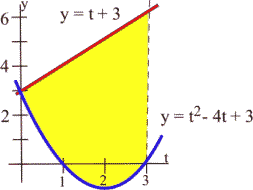
\includegraphics[width=0.3\textwidth]{img/chap5/image051.png}
    \caption{Graph for example \ref{ex:5-8-4}.}
    \label{fig:5-8-ex4}
\end{figure}

\begin{solution}

Since $v_A(t)\geq v_B(t)$, the area between the graphs of $v_A(t)$ and $v_B(t)$ represents the distance between the objects.

After 3 seconds, the distance apart is
\begin{align*}
\int_0^3(v_A(t)-v_B(t))\,dt &= \int_0^3((t+3)-(t^2-4t+3))\,dt \\
  &= \int_0^3(5t-t^2)\,dt \\
  &= \left.5\frac{t^2}{2}-\frac{t^3}{3}\right|_0^3 \\
  &= \left(5\cdot\frac{9}{2} - \frac{27}{3}\right)-(0)\\
  &= 13.5 \text{meters}.
\end{align*}
\end{solution}\end{example}

\subsection{Volume}
Just as we can partition an interval and imagine approximating an area with rectangles to find a formula for the area between curves, we can partition an interval and imagine approximating a volume with simple shapes to find a formula for the volume of a solid. While this approach works for a variety of shapes, our focus will be on shapes formed by revolving a curve around the horizontal axis.

We start with an area, the region below a function on the interval $a\leq x\leq b$ (Figure \ref{fig:5-8-region}). We are going to take that region, and rotate it around the $x$-axis, creating the solid shape shown in Figure \ref{fig:5-8-solid}.

\begin{figure}[!ht]
  \centering
    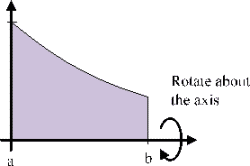
\includegraphics[width=0.3\textwidth]{img/chap5/image070.png}
    \caption{Region to rotate around the $x$-axis.}
    \label{fig:5-8-region}
\end{figure}
\begin{figure}[!ht]
  \centering
    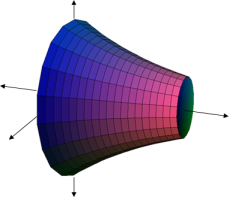
\includegraphics[width=0.3\textwidth]{img/chap5/image052.png}
    \caption{Solid formed by rotating the region.}
    \label{fig:5-8-solid}
\end{figure}
To find the volume of the solid in Figure \ref{fig:5-8-solid}, we can start by partitioning the interval $[0,1]$ and approximating the area with rectangles. As before, the width of each rectangle is $\Delta x$ and the height is $f(c_i)$.

\begin{figure}[!ht]
  \centering
    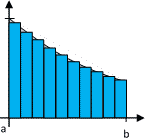
\includegraphics[width=0.3\textwidth]{img/chap5/image071.png}
    \caption{Rectangles to approximate the region.}
    \label{fig:5-8-region}
\end{figure}
\begin{figure}[!ht]
  \centering
    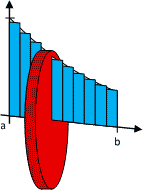
\includegraphics[width=0.3\textwidth]{img/chap5/image072.png}
    \caption{Solid formed by rotating a rectangle.}
    \label{fig:5-8-solid}
\end{figure}
If we took just one of these rectangles and rotated it about the horizontal axis, it would form a cylindrical shape. The radius of that cylinder would be $f(c_i)$, so the volume would be
$$V = \pi r^2 h = \pi(f(c_i))2\Delta x \enspace .$$
The volume of the whole solid could be approximated by rotating each of the rectangles about the $x$ axis. Adding up the volume of each of the little cylindrical discs gives an approximation of the total volume as $\displaystyle\sum_{i=1}^n \pi (f(c_i))^2\Delta x$, a Riemann sum.

The limit of this sum as the width of the rectangles becomes small is the definite integral $\displaystyle\int_a^b \pi(f(x))^2\,dx.$

\begin{theorem}[Volume]\index{Volume}
If $f(x)\geq 0$ over the interval $[a b]$, then the volume of the solid obtained by rotating about the $x$-axis the area bounded by the curve $y=f(x)$, the $x$-axis, $x=a$, and $x=b$ is
$$\int_a^b \pi(f(x))^2\,dx \enspace .$$
\end{theorem}
\begin{example}
Find the volume of the solid formed by rotating the area under the curve $y=f(x)=e^{-x}$ on the interval $[0,1]$ about the $x$-axis.

\begin{figure}[!ht]
  \centering
    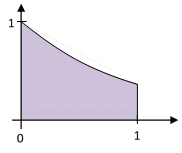
\includegraphics[width=0.3\textwidth]{img/chap5/image073.png}
    \caption{$e^{-x}$ over $[0,1]$.}
    \label{fig:5-8-enegx}
\end{figure}

\begin{solution}
This is the region pictured in the earlier example. We substitute in the function and bounds into the formula we derived to set up the definite integral:
$$\text{Volume} = \int_0^1 \pi (e^{-x})^2\,dx \enspace .$$
Using exponent rules, the integrand can be simplified. The constant $\pi$ can be pulled out of the integral:
$$\text{Volume} = \pi\int_0^1e^{-2x}\,dx \enspace .$$
Using the substitution $u=-2x$ and $du = -2\,dx$ we can integrate this function.
\begin{align*}
\pi \int_0^1 e^{-2x}\,dx &= \pi\int_{x=0}^{x=1}-\frac{1}{2}e^u\,du\\
  &= \left.-\frac{1}{2}\pi e^u\right|_{x=0}^{x=1} \\
  &= \left.-\frac{1}{2}\pi e^{-2x}\right|_0^1\\
    \left(-\frac{1}{2}\pi e^{-2(1)}\right)-\left(-\frac{1}{2}\pi e^{-2(0)}\right) \\
  &\approx 1.358 \text{ cubic units}.
\end{align*}
\end{solution}\end{example}
